\documentclass[a4paper,11pt,titlepage]{jsarticle}


% 数式
\usepackage{amsmath,amsfonts}
\usepackage{bm}
\usepackage{physics}
% 画像
\usepackage[dvipdfmx]{graphicx}
\usepackage[hang,small,bf]{caption}
\usepackage[subrefformat=parens]{subcaption}
\captionsetup{compatibility=false}

% ローマ数字
\usepackage{otf}
% 単位
\usepackage{siunitx}
% 表
\usepackage{multirow}
% 化学反応
\usepackage[version=4]{mhchem}
\usepackage{url}

\begin{document}

\title{特別実験レポート\\「タンブリングしない大腸菌集団のガラス転移」}
\author{05-211525 齋藤駿一}
\date{\today}
\maketitle

\section{序論}

ガラス転移とは,通常の液体だったものがガラス状態と呼ばれる非晶質へ変化することである.
ガラス状態とは,ミクロに見れば,液体を構成する原子や分子がランダムな配置をとったまま凍結した状態である.
さらに系の構成要素としてコロイドや高分子などを考えると,単純液体のほかにも多くのソフトマターでガラス状態が実現するといえる\cite{glass}.
とくに最近では,細胞内をガラスとして捉える研究が進んでおり,細胞質のガラス転移には細胞内の代謝活性が影響することが知られている\cite{cyto1}\cite{cyto2}.
しかし,ガラス転移およびガラス状態の性質は,長年の研究にもかかわらず理論的な理解が難しく,物性物理最後の未解決問題と呼ばれる.
とくに,代謝活性のような系の非平衡性と系のガラスとしての性質との対応関係は,未だによく分かっていない.

そこで本研究では,系の構成要素として大腸菌を選び,それらのアクティブな動きが大腸菌集団全体のガラスとしての性質にどう影響を与えるのかという問題に取り組んだ.
具体的には,カバーガラス上にプリントされた円形の井戸の中に閉じ込められた大腸菌の集団が密度の増加によってガラス転移する様子を,光学顕微鏡で観察した.
その際,大腸菌集団全体に均質に培地が行き渡るように,広域マイクロ灌流系(Extensive microperfusion system, EMPS)を用いた.
すでになされた同様の実験では,大腸菌の並進自由度と回転自由度が別々に凍結するといった興味深い現象が確認されている\cite{lama}.
本研究では,この研究と異なり,大腸菌としてランダムな方向転換(タンブリング)をしないように遺伝子操作を施された変異株を用いた.
以前Hisay Lama氏が,そのような変異株としてRP4979を用いた実験を行ったが,適切に細胞分裂せずに肥大化(繊維状に成長)する個体が出現するという問題が起こった.
そこで本研究では,UU2806,UU2864という別の変異株を用いて実験を行った.
その結果,UU2864を適切な条件で観察することによって,この大腸菌の成長の問題の解消に成功した.
本レポートではウェル内での大腸菌の成長の観察結果をまとめるにとどめ,得られた実験データの解析は今後の課題とした.

\section{方法}
\subsection{細菌の培養}
大腸菌の株としてUU2806,UU2864の2種類を用いた.
これらは,遺伝子操作によりタンブリングを制限された変異株である.
まず,これらの株のグリセロールストックを,試験管に入った\SI{5}{\mL}のLuria-Bertani (LB)培地(bacto-tryptone \SI{10}{\g/\L},NaCl \SI{10}{\g/\L},yeast \SI{5}{\g/\L})中に移した.
この試験管を,インキュベーター内(温度\SI{37}{\degreeCelsius},振動速度\SI{200}{rpm})で17~19時間ほど培養した.
次に,培養した菌液のうち\SI{50}{\uL}を,別の試験管に入った\SI{5}{\mL}のTryptone broth(TB)培地(bacto-tryptone \SI{10}{\g/\L},NaCl \SI{5}{\g/\L})に移した.
この試験管を,インキュベーター内(同温度同振動速度)で2時間培養した.
こうして得た菌液の波長\SI{600}{\nm}におけるOD(optical density)を測定した.
ODの値が大きすぎる場合は,$\mathrm{OD}_{\SI{600}{\nm}}\approx 0.1$となるように,Tween-20を\SI{0.8}{wt\%}含むTB培地を用いて希釈した.

\subsection{マイクロ流路デバイスの作製}

\begin{figure}[htbp]
  \centering
  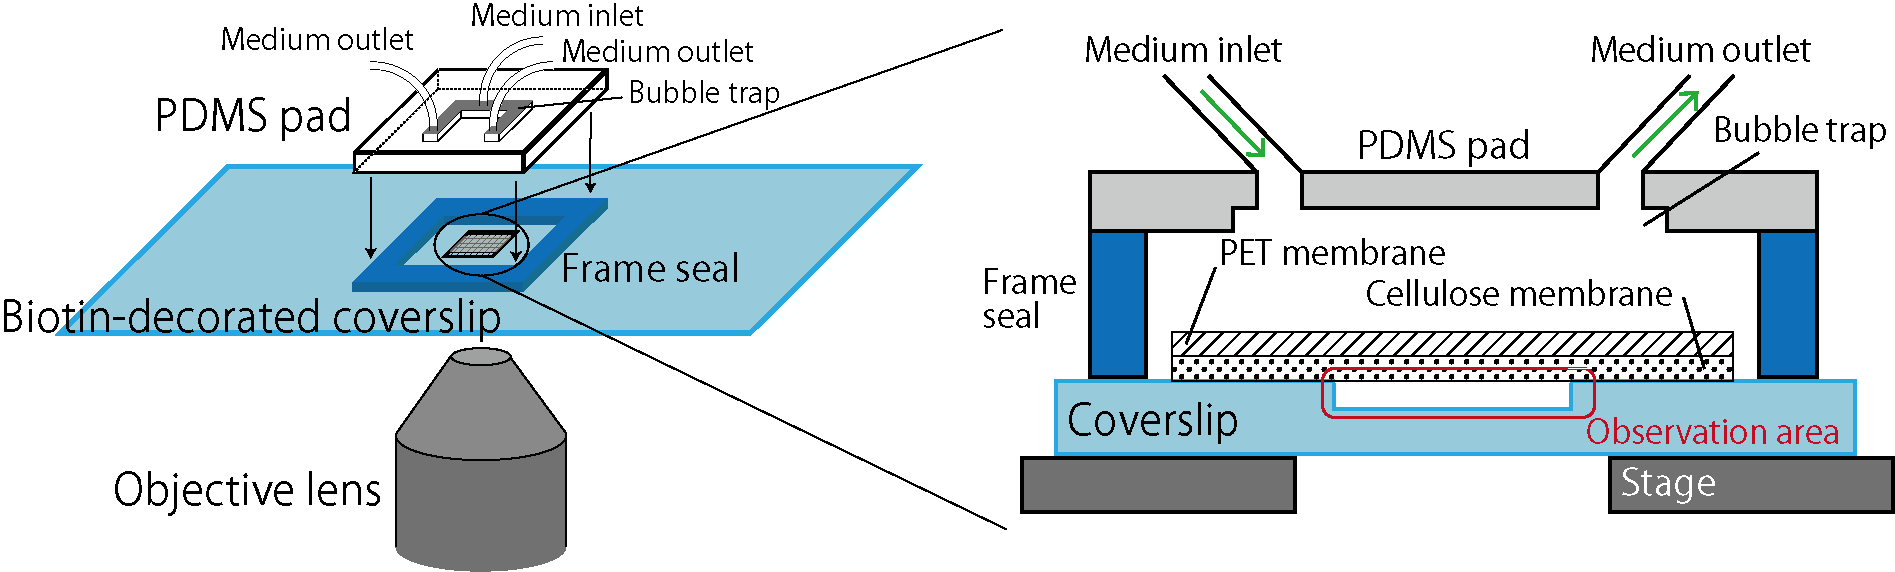
\includegraphics[width=13cm]{EMPS.png}
  \caption{広域マイクロ灌流系の模式図\cite{emps}.}
  \label{fig:EMPS}
\end{figure}

広域マイクロ灌流系は,微細加工したカバーガラスのくぼみ上にセルロース膜,PET膜(細孔径\SI{0.4}{\um})を重ね,さらにその上にPDMS製のパッドを載せた系である(図\ref{fig:EMPS}).
後述するように,あらかじめセルロース膜にはstreptavidin修飾,PET膜にはbiotin修飾を施しておき,この二枚の膜がbiotin-streptavidin結合で接着するようにしてある.
PDMSパッドには,培地の供給口と排出口が取り付けられている.

本実験では,直径\SI{120}{\um}\footnote{直径\SI{100}{\um}のつもりで作製したが,実験時にLeica LasX上で直径を測ると\SI{120}{\um}となっていた.},深さ約\SI{1.2}{\um}のくぼみ(ウェル)が多数プリントされたカバーガラスを用いた.
このカバーガラスの微細加工は,洗浄したカバーガラスにクロムを蒸着し,その上にレジストを塗布してパターン感光した後,フッ酸エッチングを施して行った.
こうして得たカバーガラスとPET膜をオルガノシラン(3-(2-aminoethyl aminopropyl) trimethoxysilane)の\SI{1}{wt\%}溶液にそれぞれ30分間,45分間浸した.
その後,PET膜を数mm四方に切り,それをカバーガラスのパターン上に載せ,その上からbiotin溶液を\SI{0.2}{\mL}垂らし,インキュベーター内(\SI{25}{\degreeCelsius})で4時間30分静置した.
また,セルロース膜にstreptavidin溶液を\SI{2}{\mL}載せてインキュベーター内(\SI{25}{\degreeCelsius})の振とう器に置き,約14時間振とうさせた.

デバイスを組み立てる際は,まずstreptavidin修飾済みのセルロース膜を数mm四方に切り,biotin修飾済みのPET膜と重ね,TB寒天円盤(\SI{1.5}{wt\%}の寒天を含むTB培地を用いて作製した)で挟み,二重膜を作製した.
次に,カバーガラスのパターン上に菌液を\SI{2}{\uL}垂らした.
その後,二重膜をTB寒天円盤から取り出し,空中で20秒ほど乾燥させてから,パターン上に載せた.
その上にTB寒天円盤を20秒間載せ,外してから10秒後にTween-20を\SI{0.8}{wt\%}含むTB培地を\SI{3}{\uL}垂らした.
最後にPDMS製のパッドを両面テープ(図\ref{fig:EMPS}の濃い青色の部分)で接着してカバーガラス上に固定した.

\subsection{細菌の観察}
EMPSデバイスを倒立光学顕微鏡Leica DMi8のステージに固定し,63x($\mathrm{NA}=1.30$)の油浸対物レンズを用いて観察した.
顕微鏡の操作にはソフトウェアLeica LasXを用いた.
実験中はつねにTween-20を\SI{0.8}{wt\%}含むTB培地がPDMS製パッドの供給口から供給されるようにした.
培地の供給にはシリンジポンプNE-1000を用いた.
供給速度は,実験開始直後は\SI{50}{\mL/h},累計\SI{5}{\mL}が供給された後は\SI{2}{\mL/h}となるように設定した.
また,観察中はカバーガラスの温度を\SI{30}{\degreeCelsius}に保った.

\section{結果と考察}

\subsection{UU2806を用いた実験}
\subsubsection{結果}

\begin{figure}[htbp]
  \centering
  \begin{minipage}{0.45\linewidth}
    \centering
    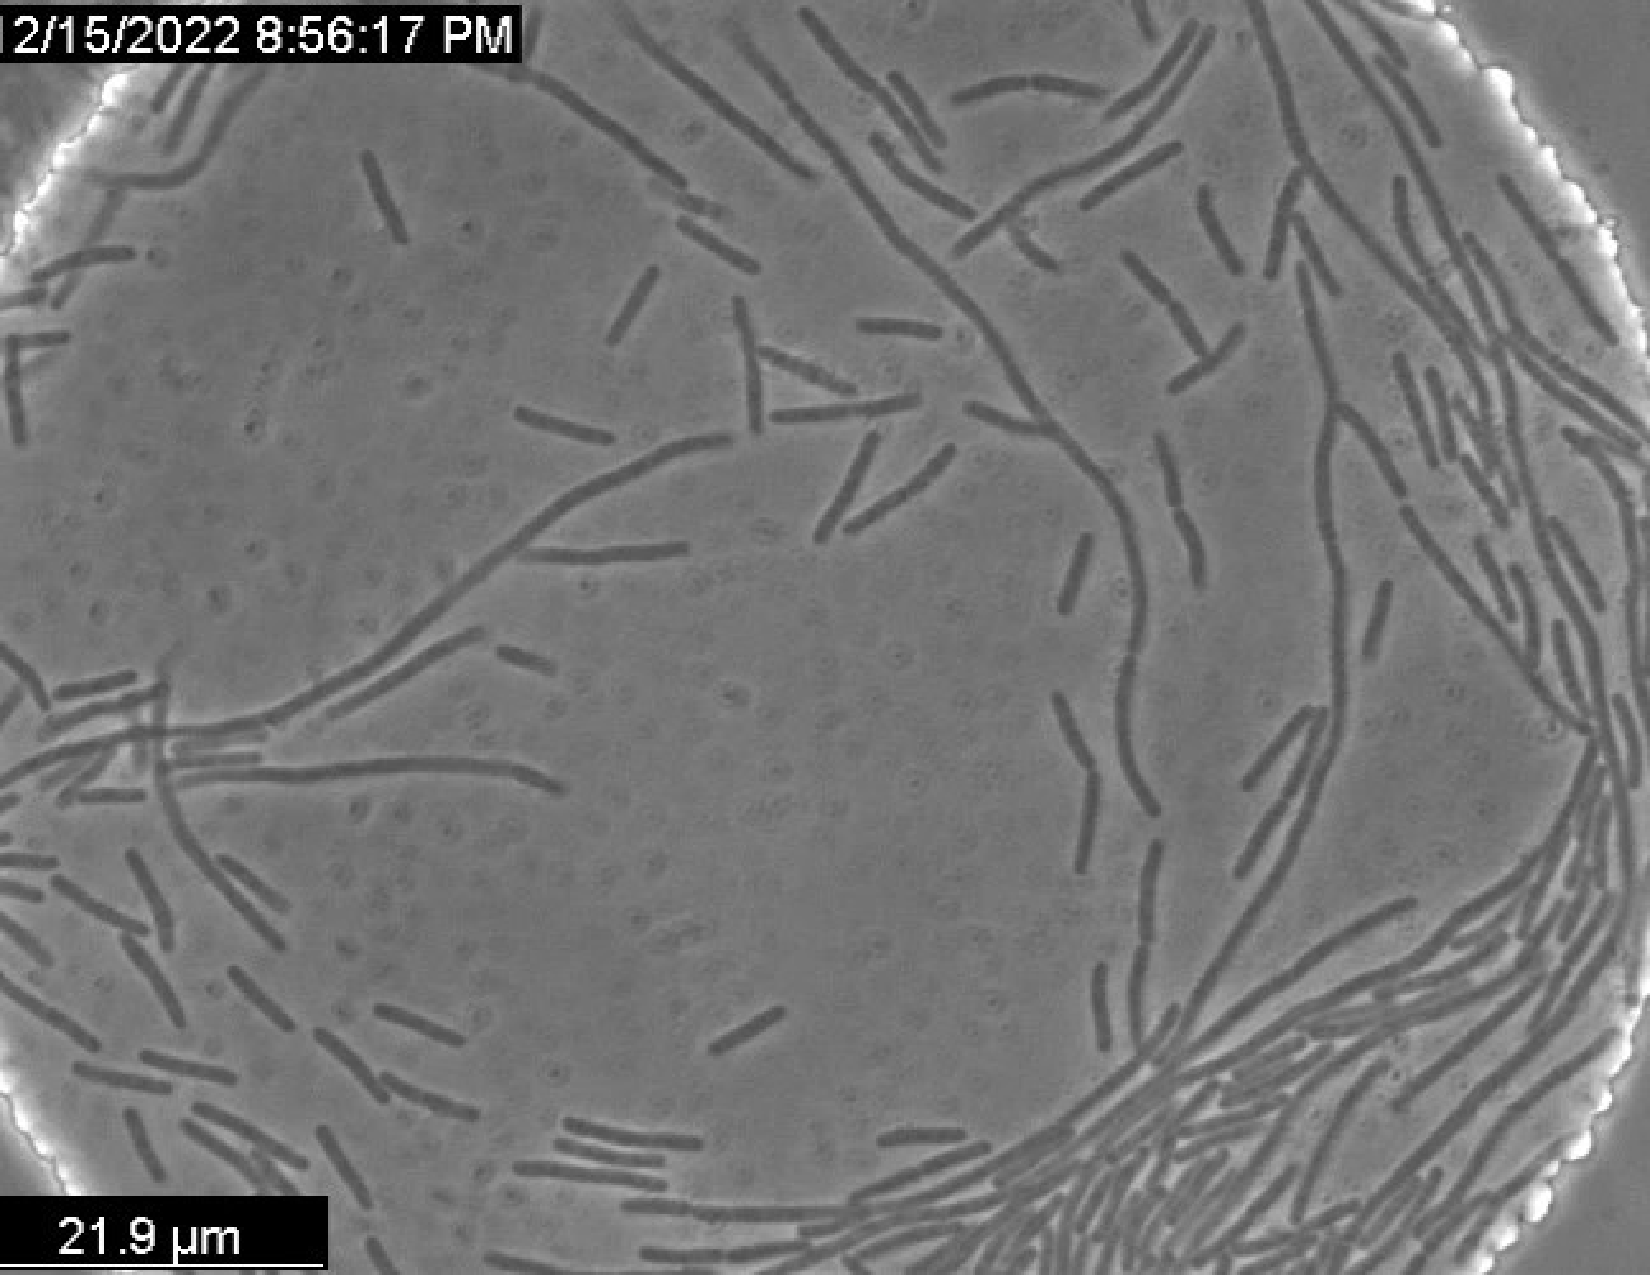
\includegraphics[width=\columnwidth]{Series015_t060000_RAW_ch00.pdf}
    \subcaption{菌液注入から約6時間後.}
    \label{fig:06_1}
  \end{minipage}
  \begin{minipage}{0.45\linewidth}
    \centering
    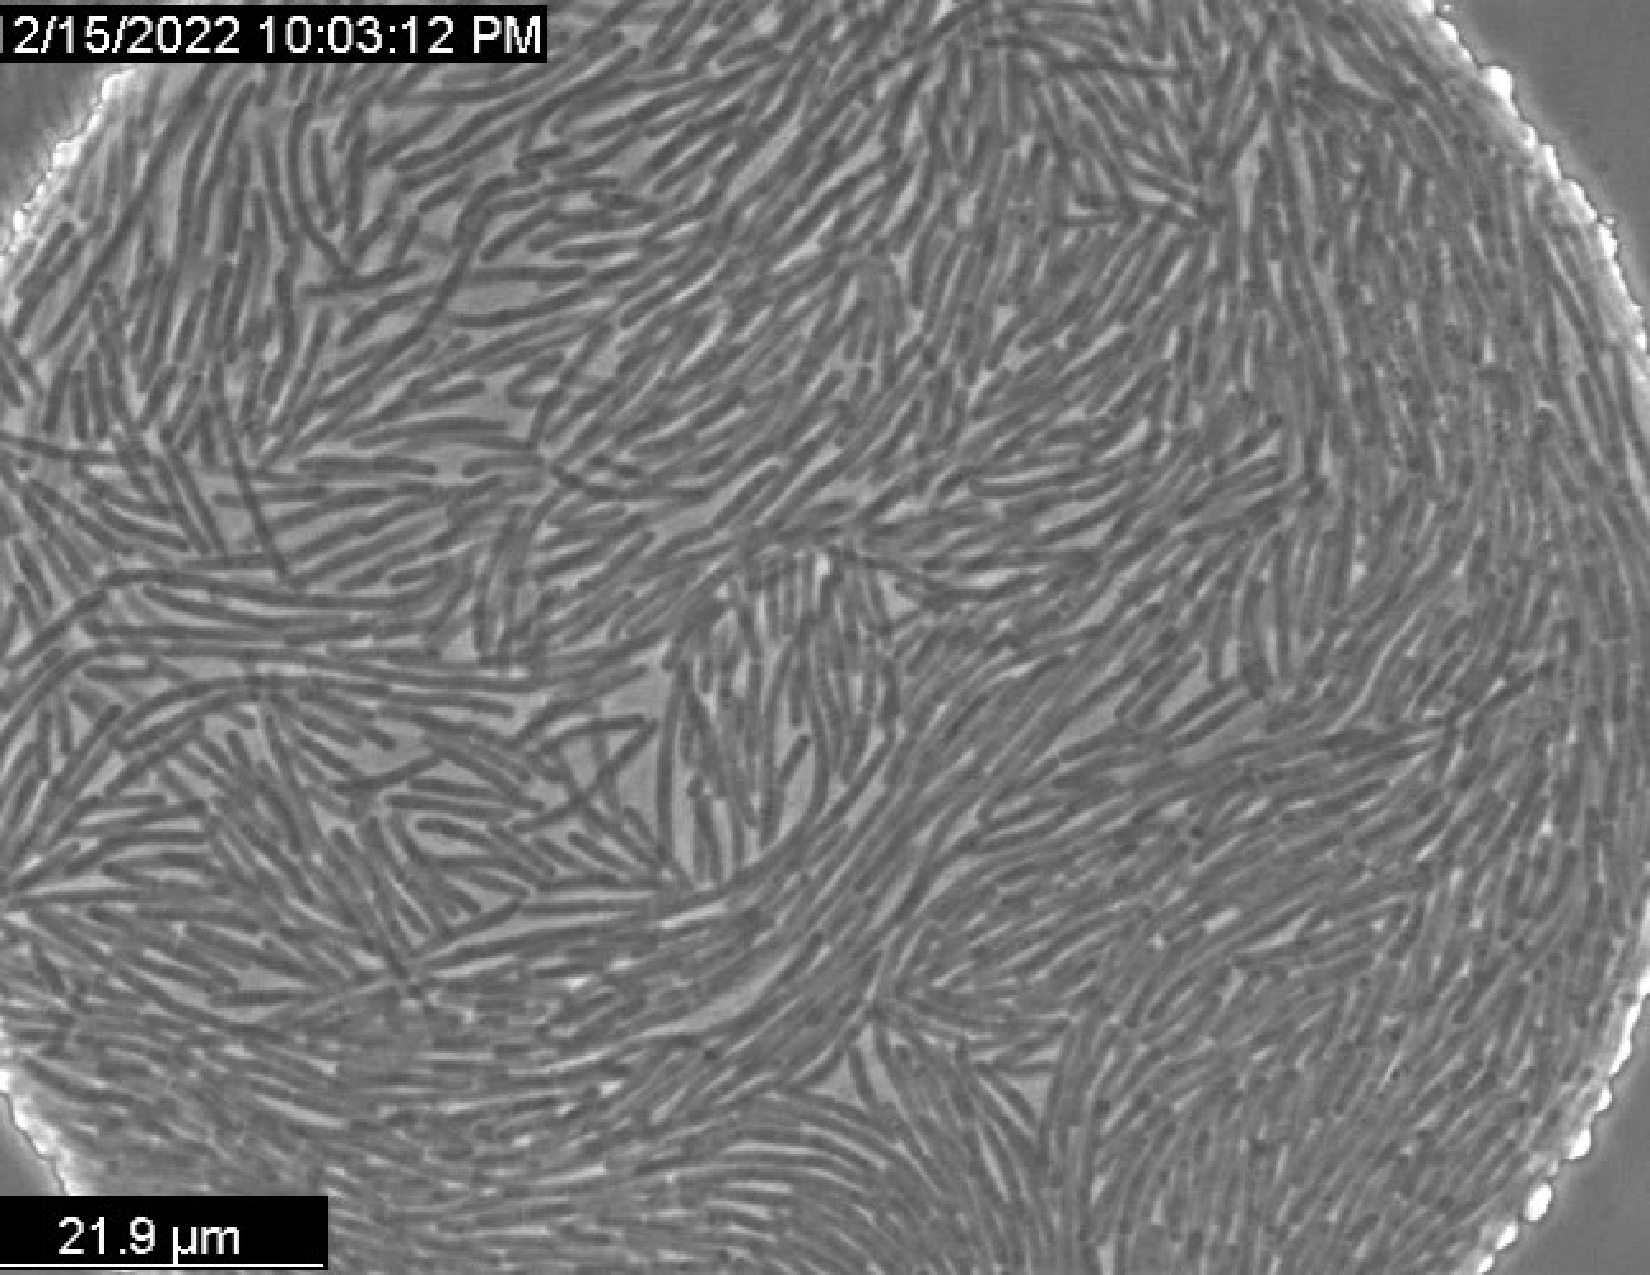
\includegraphics[width=\columnwidth]{Series015_t100000_RAW_ch00.pdf}
    \subcaption{菌液注入から約7時間10分後.}
    \label{fig:06_2}
  \end{minipage}
  \begin{minipage}{0.45\linewidth}
    \centering
    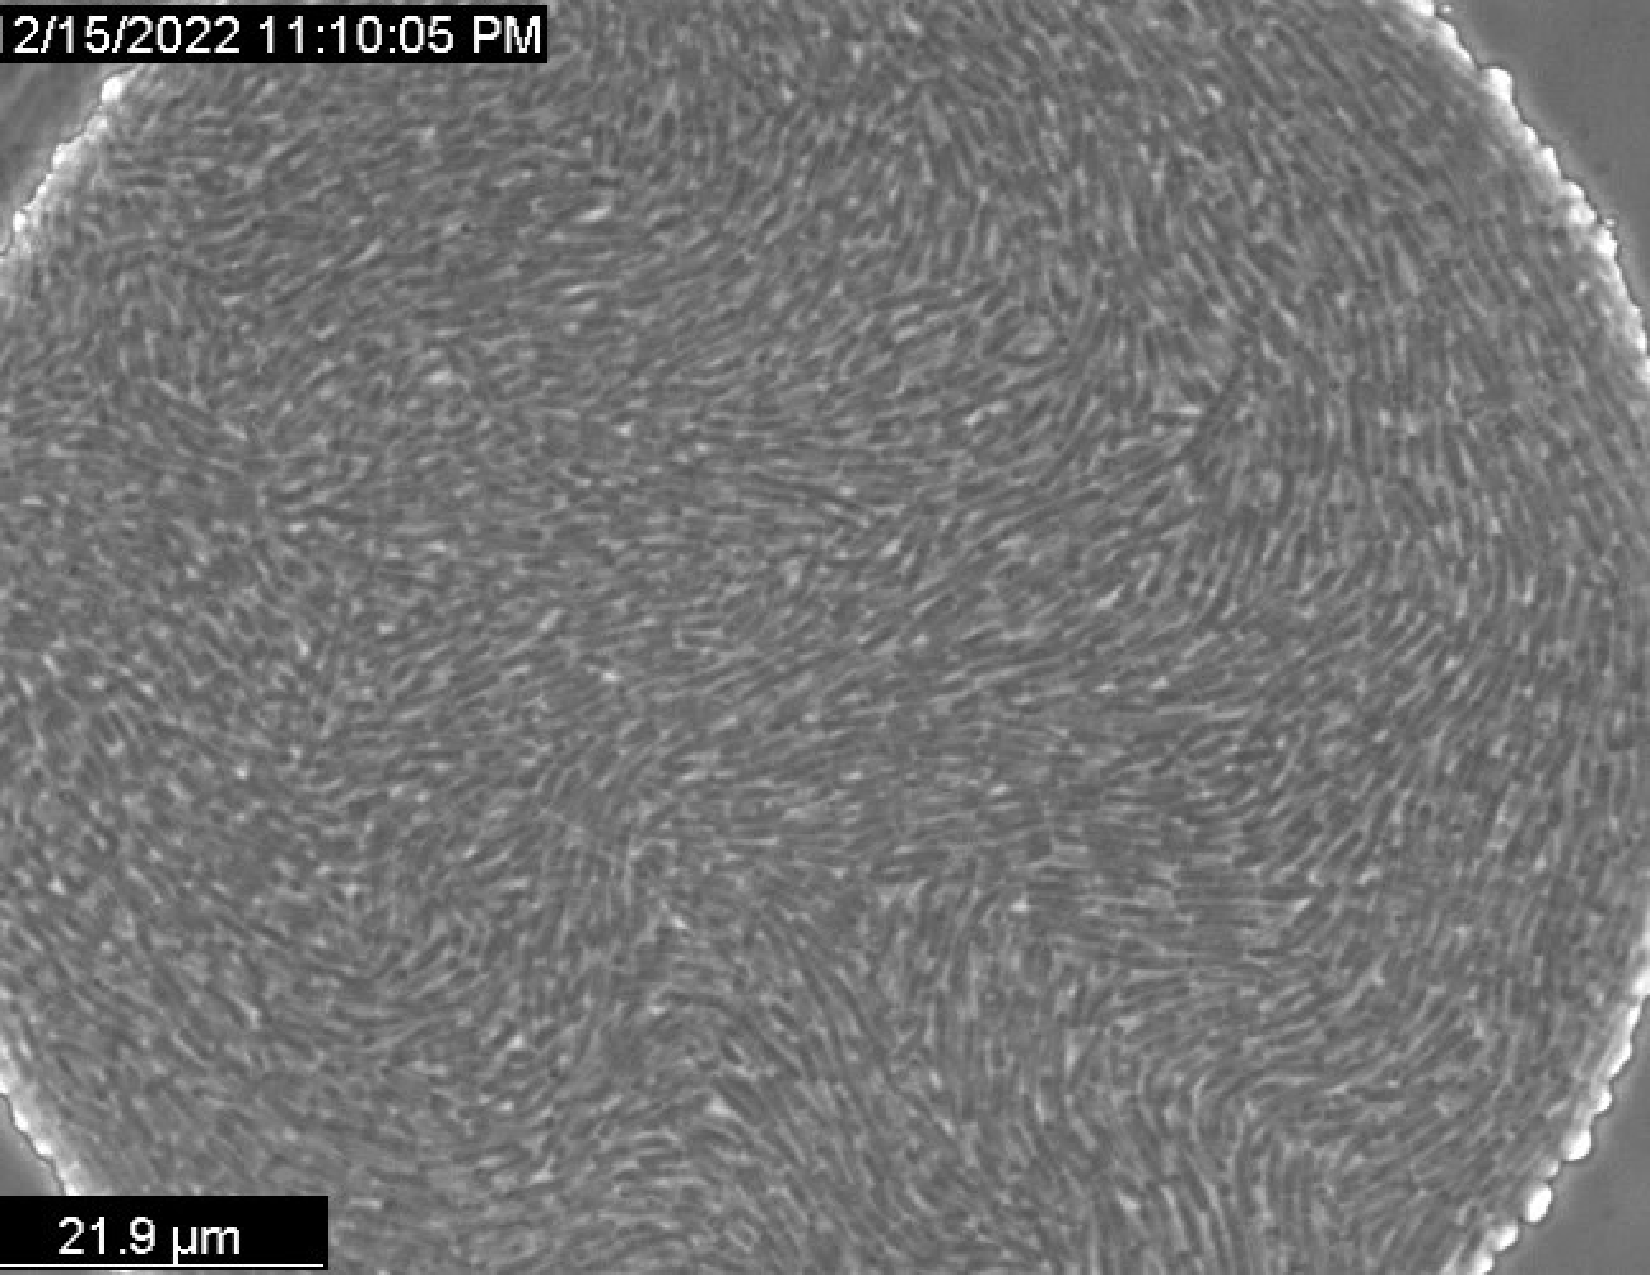
\includegraphics[width=\columnwidth]{Series015_t140000_RAW_ch00.pdf}
    \subcaption{菌液注入から約8時間20分後.}
    \label{fig:06_3}
  \end{minipage}
  \begin{minipage}{0.45\linewidth}
    \centering
    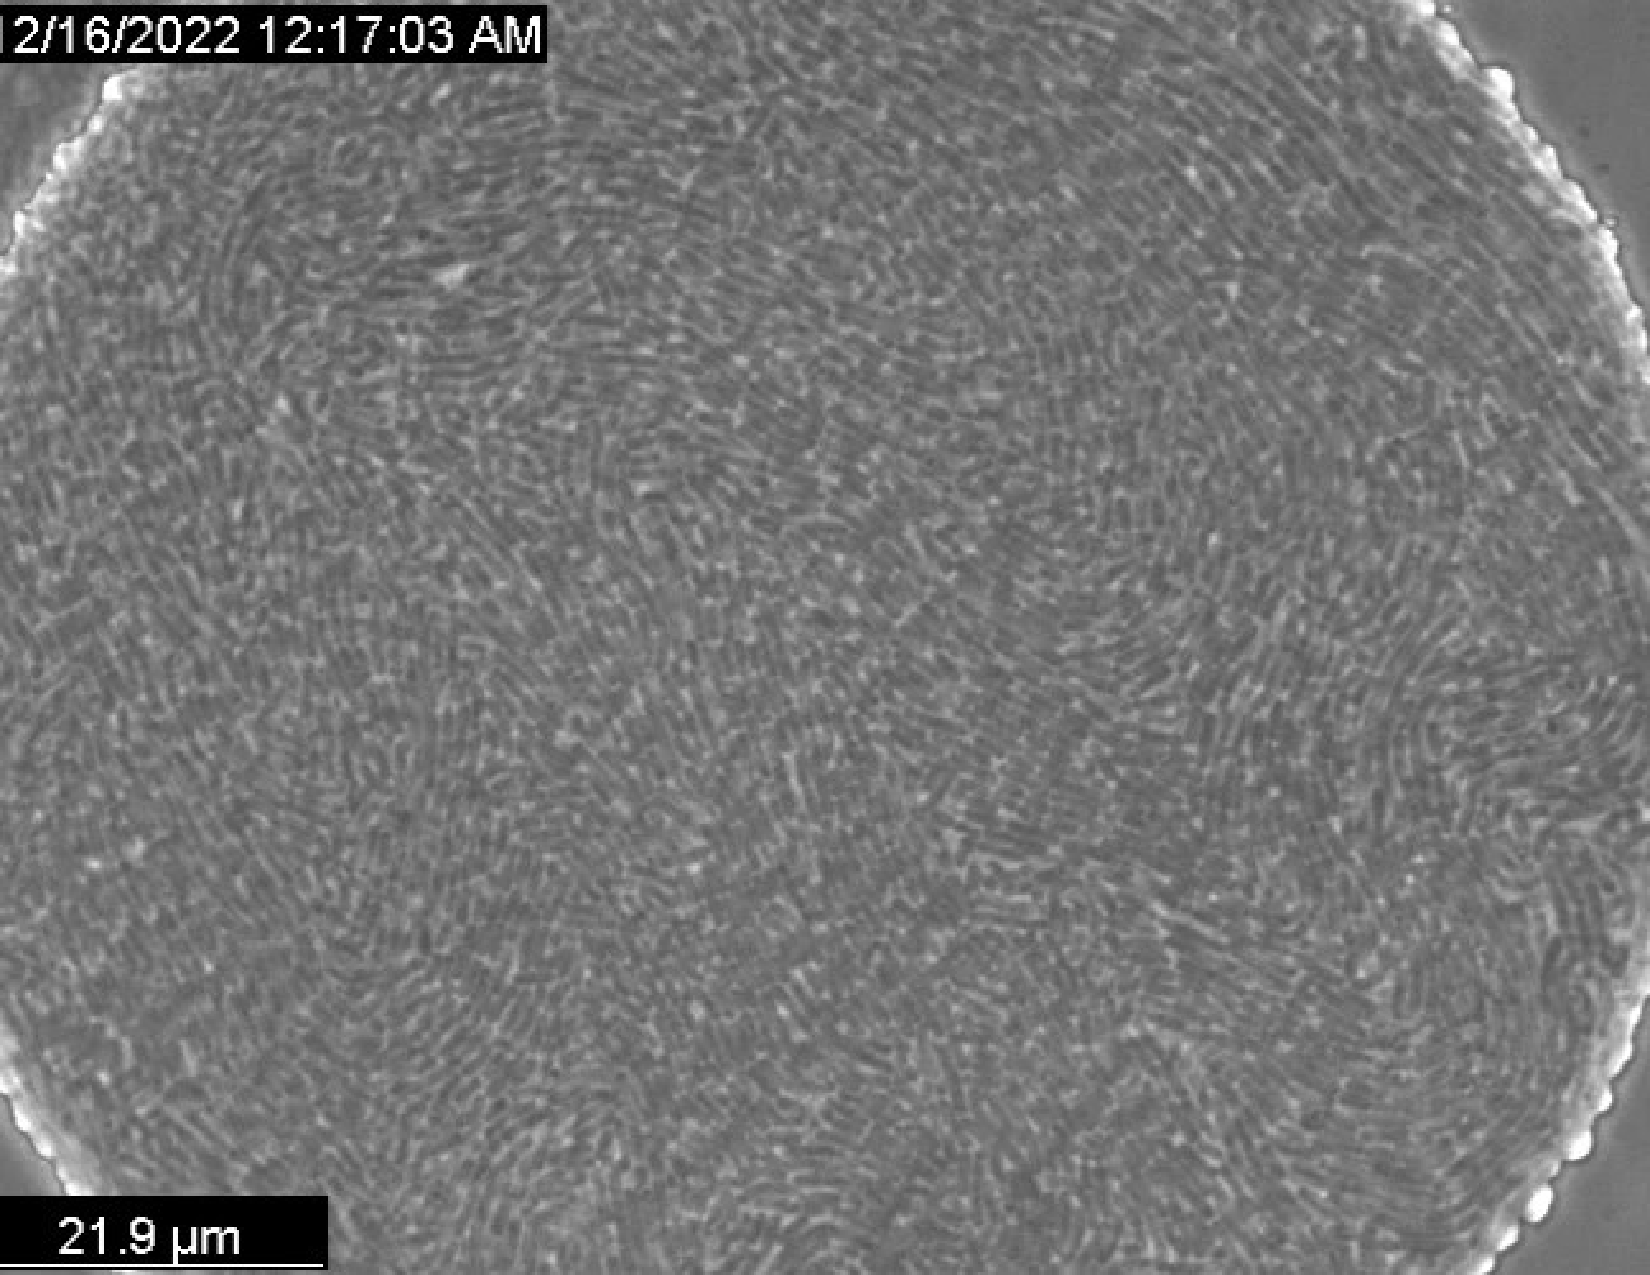
\includegraphics[width=\columnwidth]{Series015_t180000_RAW_ch00.pdf}
    \subcaption{菌液注入から約9時間20分後.}
    \label{fig:06_4}
  \end{minipage}
  \caption{UU2806を用いた実験結果.左上の時刻表示に合わせると,菌液注入の時刻は14時55分頃である.}
  \label{fig:06}
\end{figure}

UU2806を用いた実験では,2時間培養後に$\mathrm{OD}_{\SI{600}{nm}}=0.088$となっていた菌液を希釈せず用いた.
観察の結果,まず菌液をウェルに注入してから約6時間後には,ウェルの境界に吸着した数匹の個体が繊維状に成長していた(図\ref{fig:06_1}).
そしてこれらの繊維状の個体は,正常に分裂した個体の集団に押されて位置を固定され,ガラス転移が進んだ(図\ref{fig:06_2}).
ガラス転移の進行に伴って菌はほぼ静止し,繊維状の個体は分裂したが,それらの繊維に沿った配向は残っていた(図\ref{fig:06_3}).
その後ウェルの左上から菌が漏れ出て,多くの菌が左上向きに配向した(図\ref{fig:06_4}).
このときには繊維状の個体は見られなかった.

\subsubsection{考察}

\begin{figure}[htbp]
  \centering
  \begin{minipage}{0.45\linewidth}
    \centering
    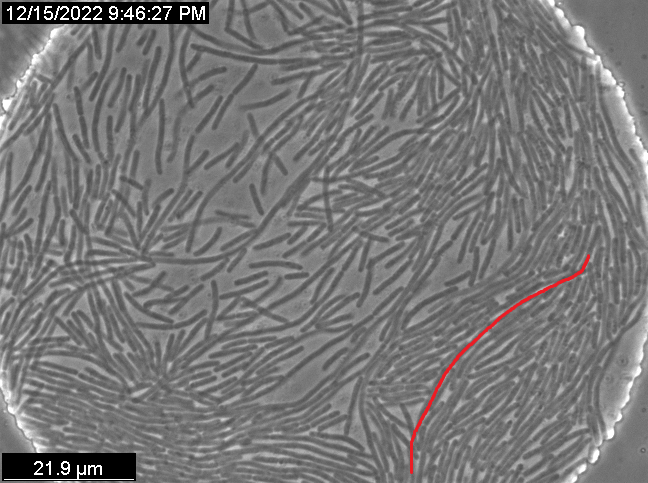
\includegraphics[width=\columnwidth]{Series015_t090000_ch00.png}
    \subcaption{菌液注入から約6時間50分後.}
    \label{fig:06_1_pt}
  \end{minipage}
  \begin{minipage}{0.45\linewidth}
    \centering
    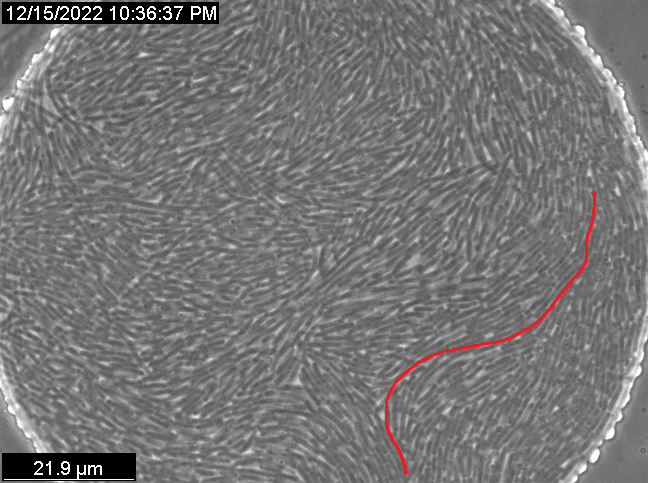
\includegraphics[width=\columnwidth]{Series015_t120000_ch00.png}
    \subcaption{菌液注入から約7時間40分後.}
    \label{fig:06_2_pt}
  \end{minipage}
  \begin{minipage}{0.45\linewidth}
    \centering
    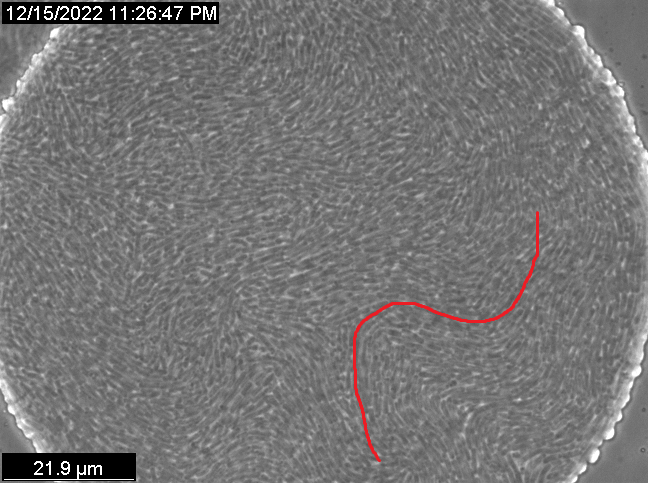
\includegraphics[width=\columnwidth]{Series015_t150000_ch00.png}
    \subcaption{菌液注入から約8時間30分後.}
    \label{fig:06_3_pt}
  \end{minipage}
  \begin{minipage}{0.45\linewidth}
    \centering
    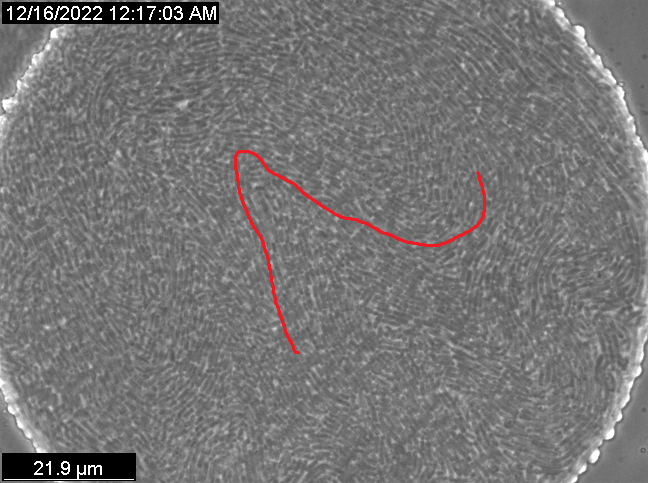
\includegraphics[width=\columnwidth]{Series015_t180000_ch00.png}
    \subcaption{菌液注入から約9時間20分後.}
    \label{fig:06_4_pt}
  \end{minipage}
  \caption{UU2806を用いた実験(図\ref{fig:06}と同じ)の結果.繊維状の個体に対応するおおよその場所を赤線で示した.}
  \label{fig:06_pt}
\end{figure}

ここでは主に,繊維状の個体がガラス状態に与える影響について考察する.
実験の結果得られた大腸菌の配向場に注目すると,繊維状の個体に沿って形成された配向がつねに保たれていることが分かった(図\ref{fig:06_1_pt},図\ref{fig:06_2_pt},図\ref{fig:06_3_pt}).
さらにこの配向は,ウェルの漏れにより大腸菌集団が左上に流れていく際も保たれていた(図\ref{fig:06_4_pt}).
この配向が生じた最大の原因は,繊維状の個体が分裂する前にガラス転移が進行したことであると考える.
逆に言えば,ガラス転移時に繊維状の個体が存在するとき,その繊維に沿った配向が形成され,それはある程度安定に持続すると考える.
そして,繊維の変形が連続変形であることから,このようなガラス転移をトポロジーの言葉で議論できることが予想される.

一方で,繊維状の個体がなぜ出現するのかについてははっきりとは考察できなかった.
また,上述したように繊維状の個体の寄与が支配的に見えるため,大腸菌がタンブリングしないことの寄与がどこに現れるかは分からなかった.


\subsection{UU2864を用いた実験}
\subsubsection{結果}

\begin{figure}[htbp]
  \centering
  \begin{minipage}{0.45\linewidth}
    \centering
    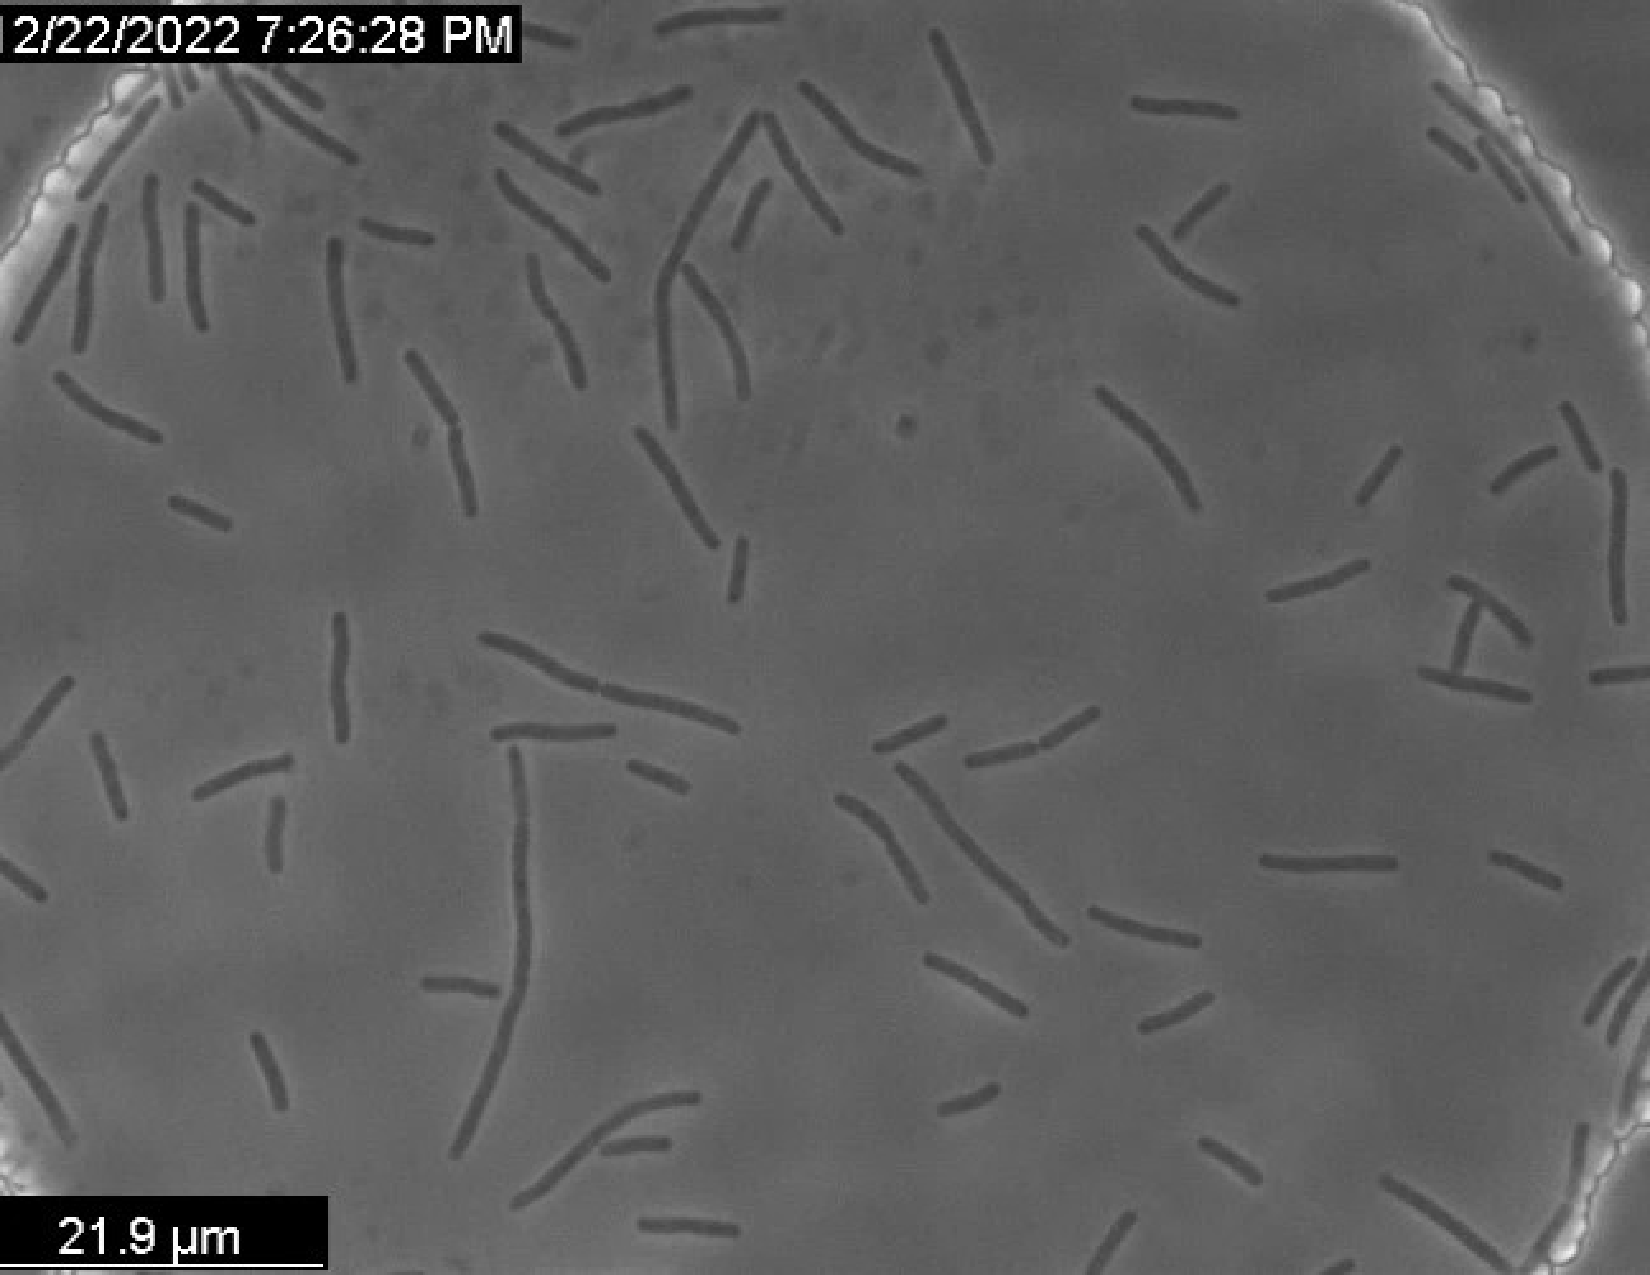
\includegraphics[width=\columnwidth]{Series007_t000000_RAW_ch00.pdf}
    \subcaption{菌液注入から約5時間20分後.}
    \label{fig:64_1}
  \end{minipage}
  \begin{minipage}{0.45\linewidth}
    \centering
    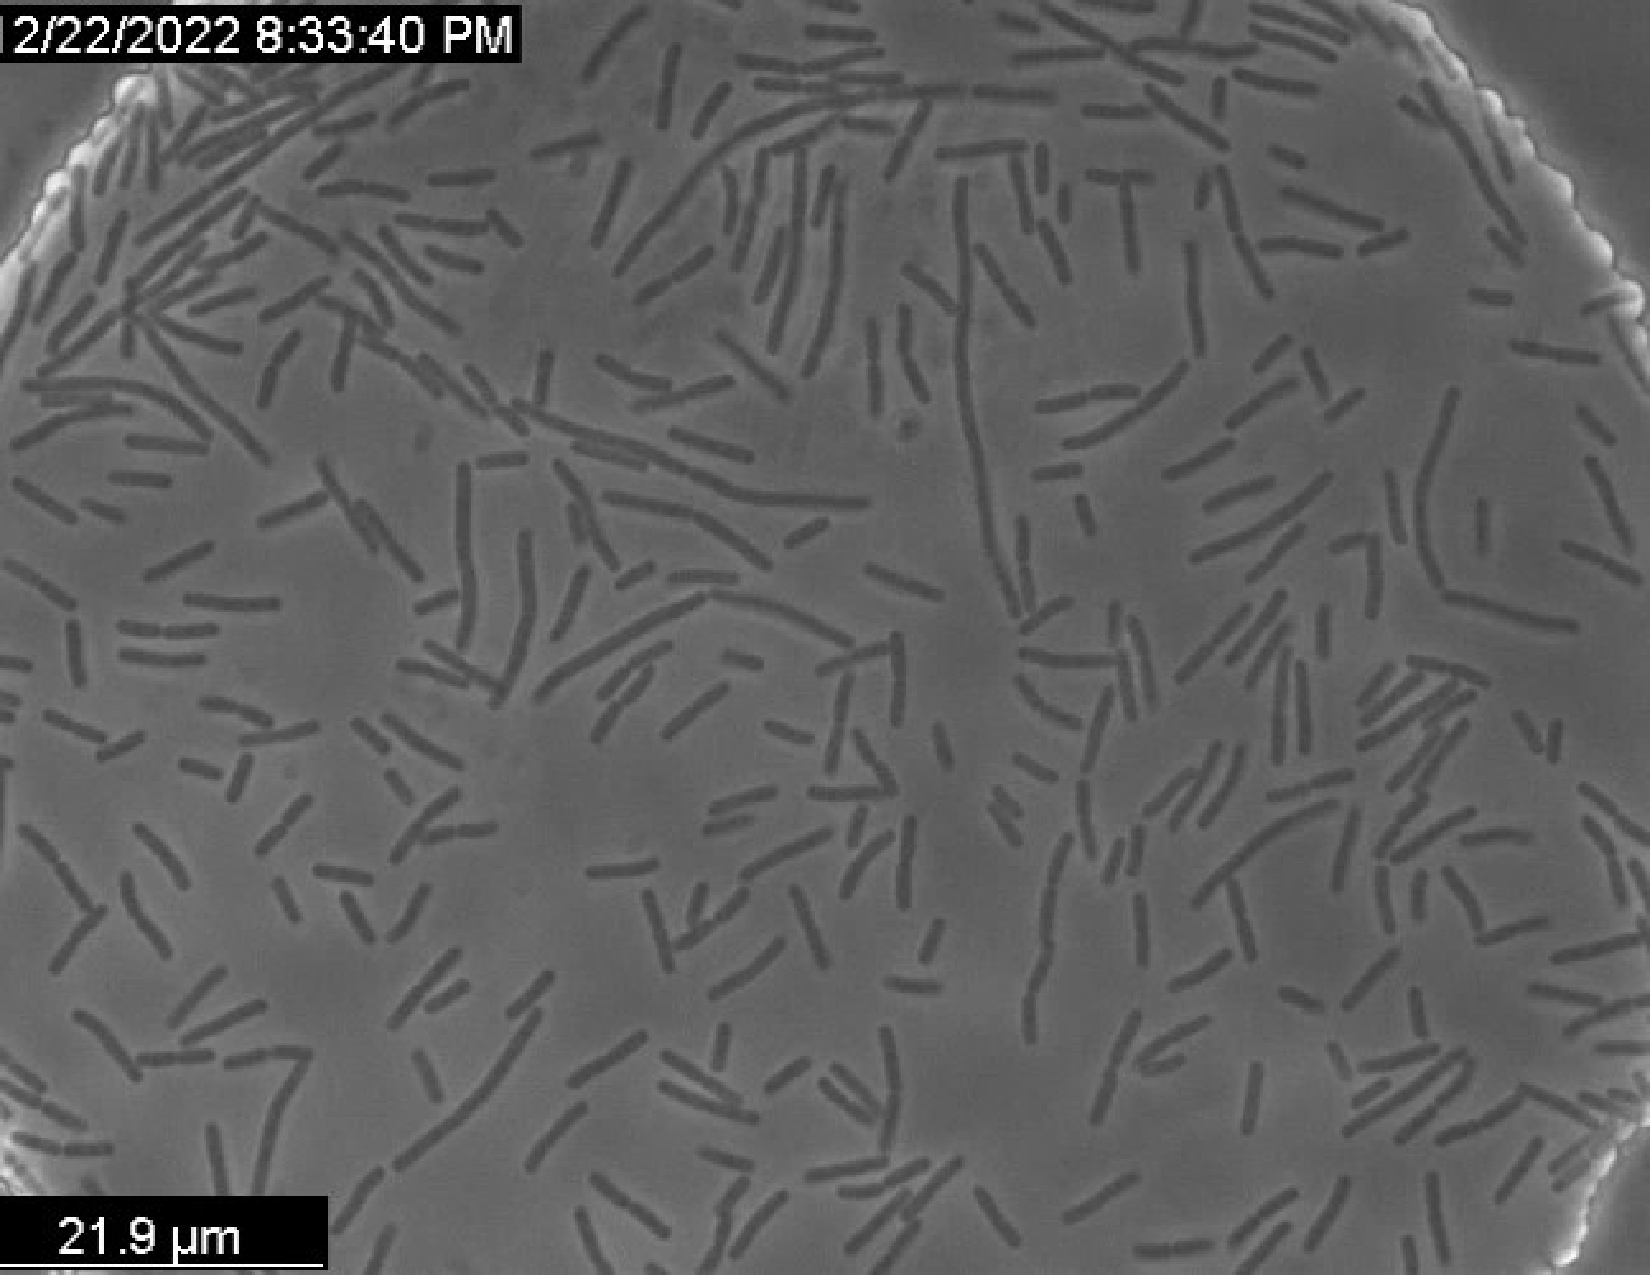
\includegraphics[width=\columnwidth]{Series007_t040000_RAW_ch00.pdf}
    \subcaption{菌液注入から約6時間30分後.}
    \label{fig:64_2}
  \end{minipage}
  \begin{minipage}{0.45\linewidth}
    \centering
    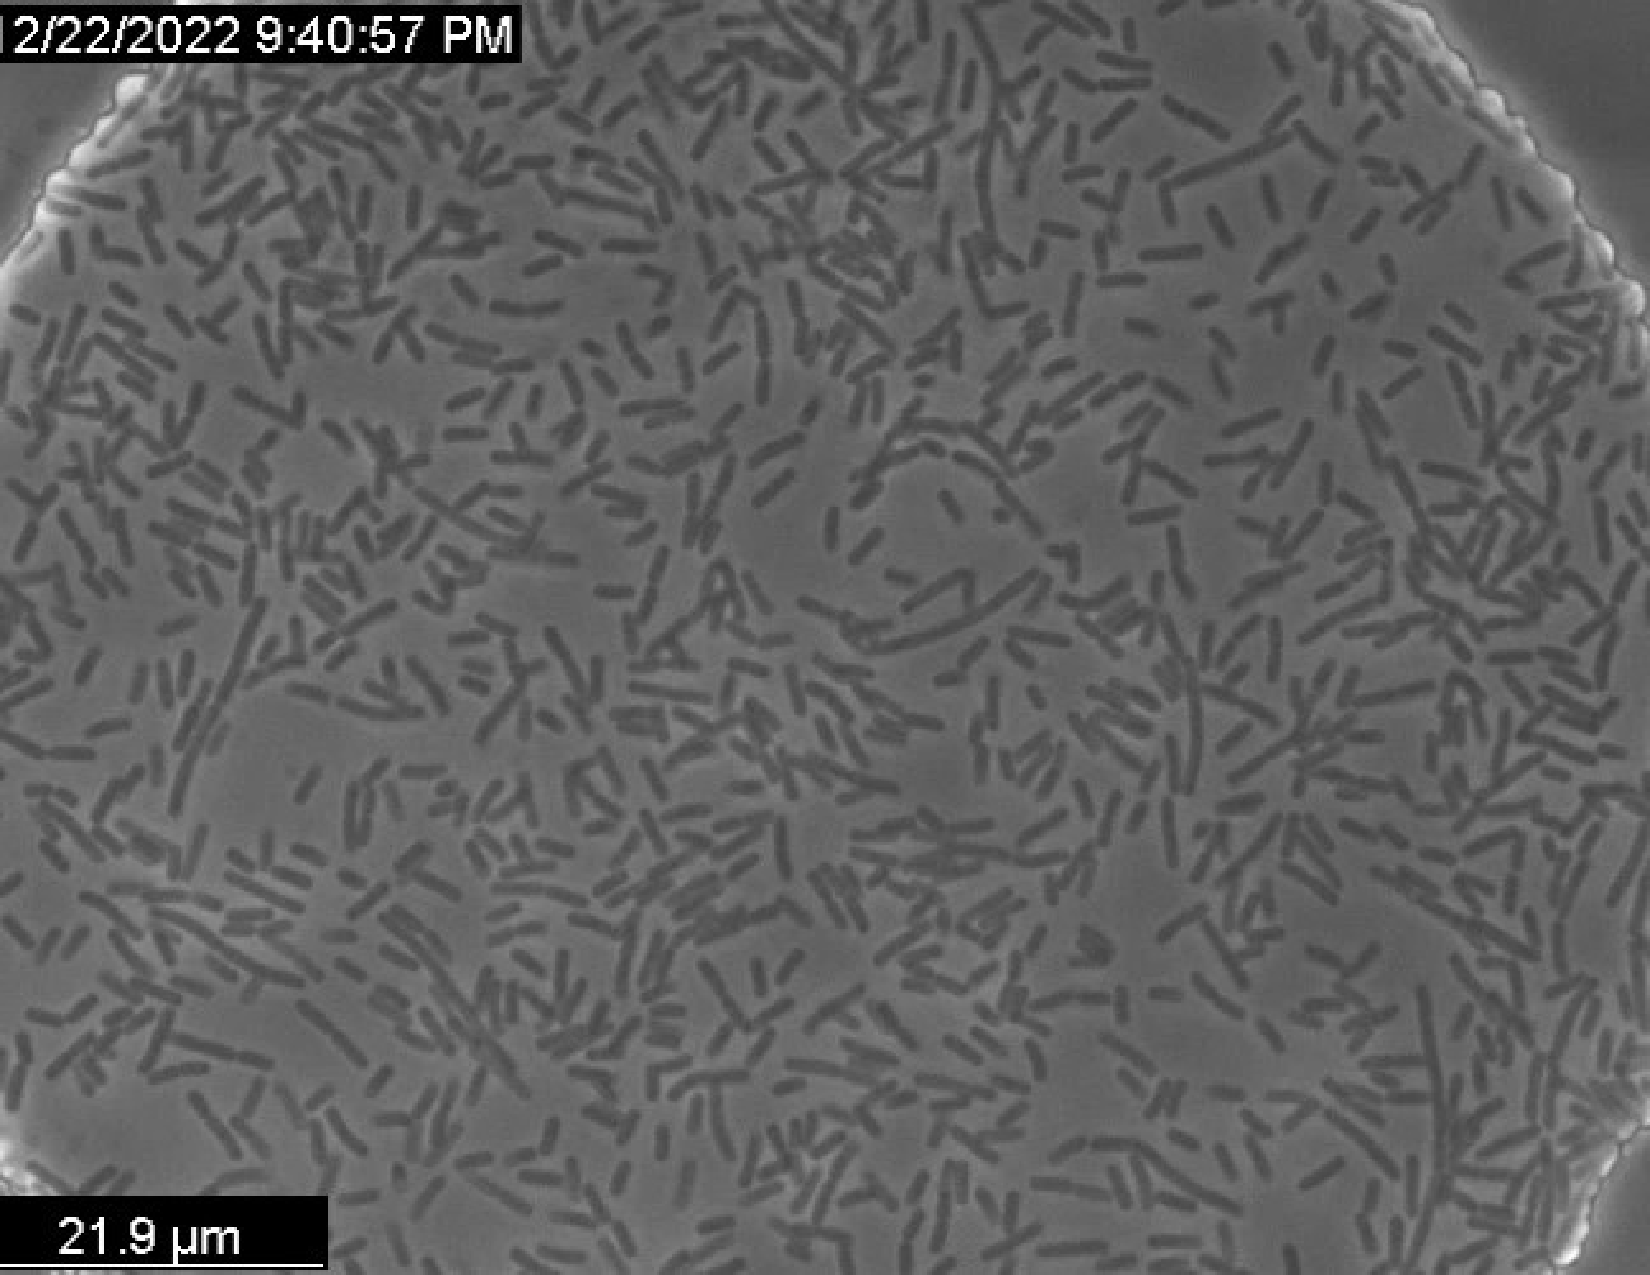
\includegraphics[width=\columnwidth]{Series007_t080000_RAW_ch00.pdf}
    \subcaption{菌液注入から約7時間40分後.}
    \label{fig:64_3}
  \end{minipage}
  \begin{minipage}{0.45\linewidth}
    \centering
    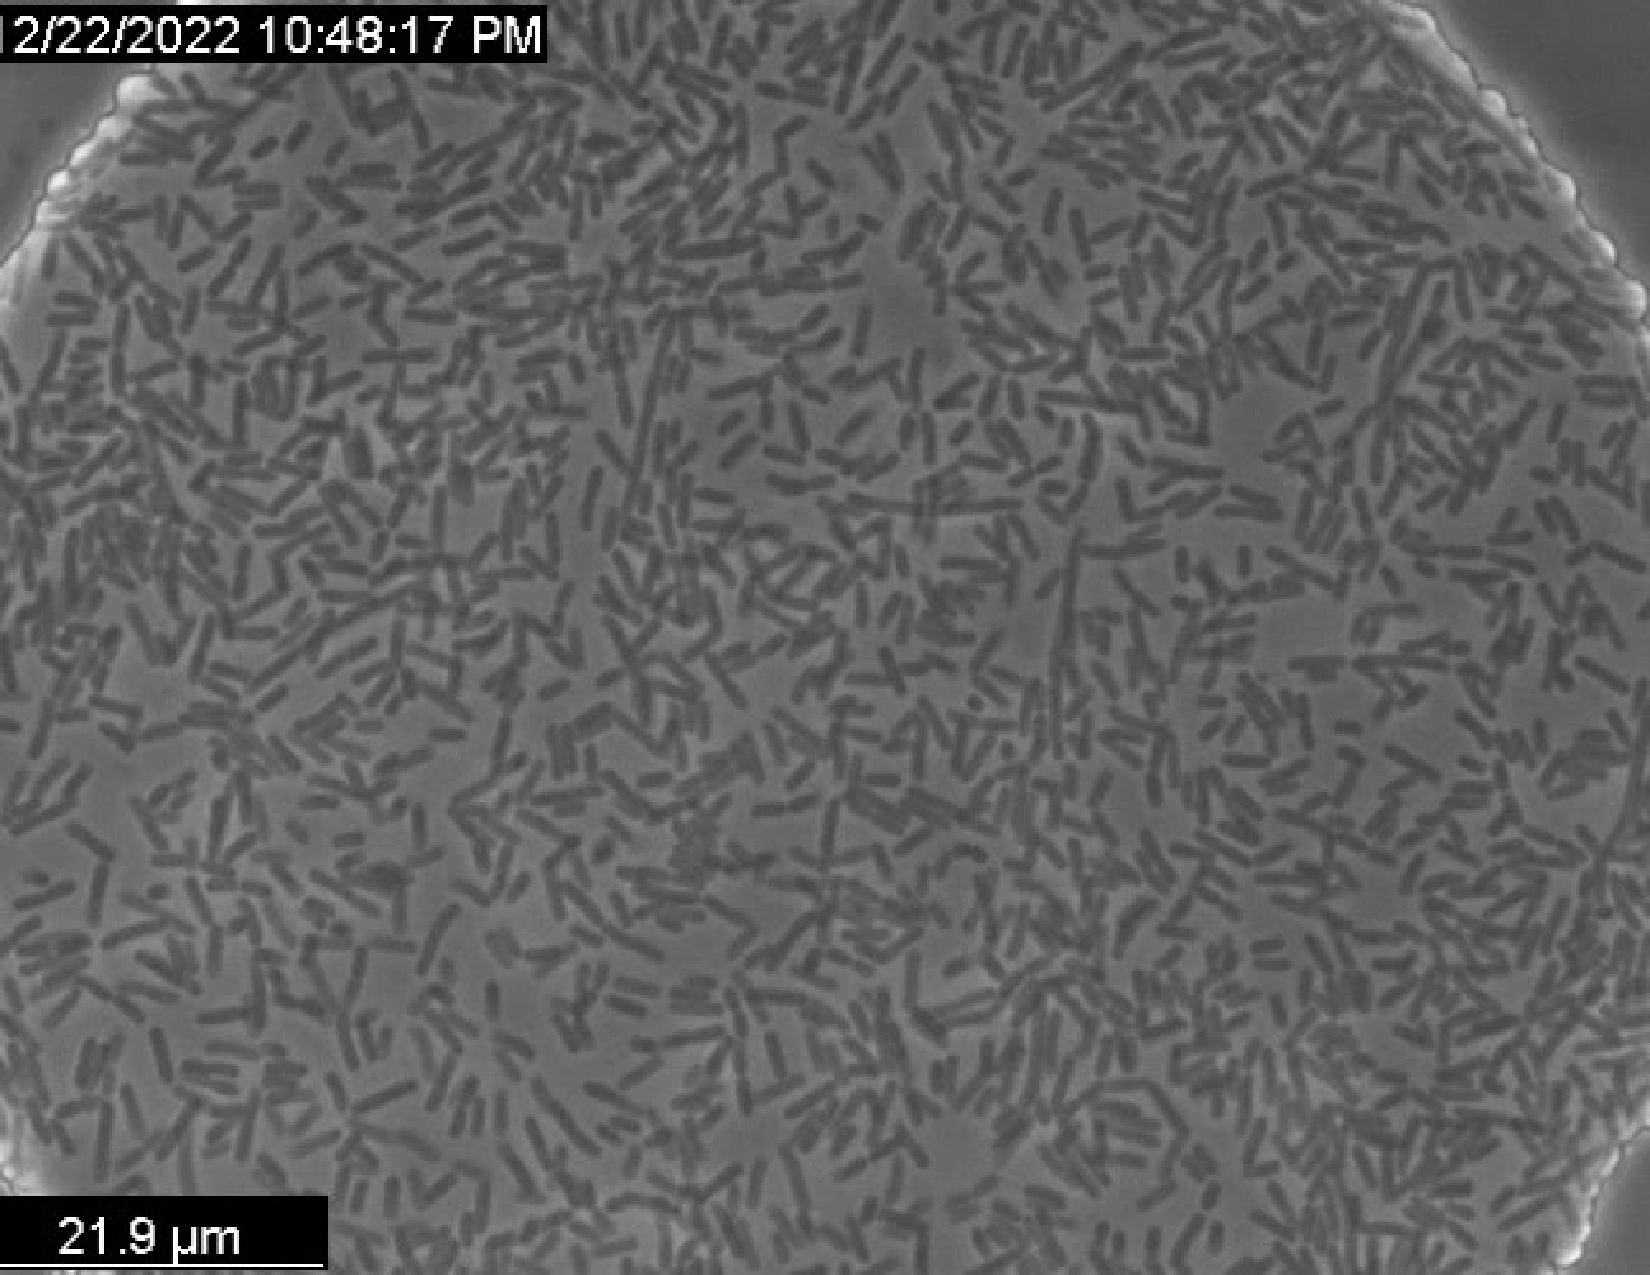
\includegraphics[width=\columnwidth]{Series007_t120000_RAW_ch00.pdf}
    \subcaption{菌液注入から約8時間50分後.}
    \label{fig:64_4}
  \end{minipage}
  \caption{UU2864を用いた実験の結果.左上の時刻表示に合わせると,菌液注入の時刻は14時3分頃である.}
\end{figure}

UU2864を用いた実験では,2時間培養後に$\mathrm{OD}_{\SI{600}{nm}}=0.243$となっていた菌液を\SI{50}{\%}に希釈して用いた.
この実験でも同様に,菌液注入から約5時間後に,繊維状に成長した個体が見られた(図\ref{fig:64_1}).
ただし,繊維の長さはUU2806の観察で見られたものより短く,それらはウェルの境界に吸着せずに動いていた.
しかし,その1,2時間後には減数分裂の割合が増え,繊維状の個体が減っていた(図\ref{fig:64_2},図\ref{fig:64_3}).
観察したウェルでは,菌液注入から9時間近く経ってもガラス転移に至らなかった(図\ref{fig:64_4}).

\subsubsection{考察}
減数分裂の起こる大きな理由として,大腸菌が飢餓状態にあることが挙げられる.
そのため,TB培地に含まれる何らかの成分が,セルロース膜に吸着するなどの理由で,大腸菌に適切に届かなかった可能性がある.
しかし,UU2806は減数分裂せずに成長しているため,別の理由で大腸菌の代謝が適切に進まなかった可能性もある.
この二つの可能性を踏まえ,次節で述べる追加実験を行った.

\section{追加実験}

\subsection{手法}
UU2864を用い,前述した手法のうち以下の点を変更して追加実験を行った.
\begin{itemize}
  \item 2時間の培養に用いる培地をTB培地ではなくM9培地(disodium phosphate (anhydrous) \SI{0.68}{wt\%},monopotassium phosphate \SI{0.3}{\%},sodium chloride \SI{0.05}{wt\%},ammonium chloride \SI{0.1}{wt\%},glucose \SI{0.2}{wt\%},\ce{MgSO4} \SI{2}{mM},\ce{CaCl2} \SI{0.1}{mM},MEM amino acids (SIGMA M5550) \SI{1}{wt\%})とした.
  \item 観察時に供給する培地,菌液を希釈する際に用いる培地,デバイスの組み立て時に\SI{3}{\uL}加える培地をいずれも,Tween-20を\SI{0.8}{wt\%}含むTB培地ではなく,Tween-20を\SI{0.8}{wt\%}含むM9培地とした.
  \item ウェルの直径を\SI{120}{\um}ではなく\SI{100}{\um}とした.
  \item カバーガラスの温度を\SI{30}{\degreeCelsius}ではなく\SI{37}{\degreeCelsius}に保った.
\end{itemize}
ここでM9培地を用いた理由は,その組成が明確に定まっており,問題の原因となったTB培地の成分を含まないと考えたからである.
また,カバーガラスの温度を\SI{37}{\degreeCelsius}にした理由は,それが大腸菌の最適な培養温度だからである.
さらに,ウェルの直径を小さくすることで,ガラス転移までの時間を短縮できると考えた.

\subsection{結果と考察}

\begin{figure}[htbp]
  \centering
  \begin{minipage}{0.45\linewidth}
    \centering
    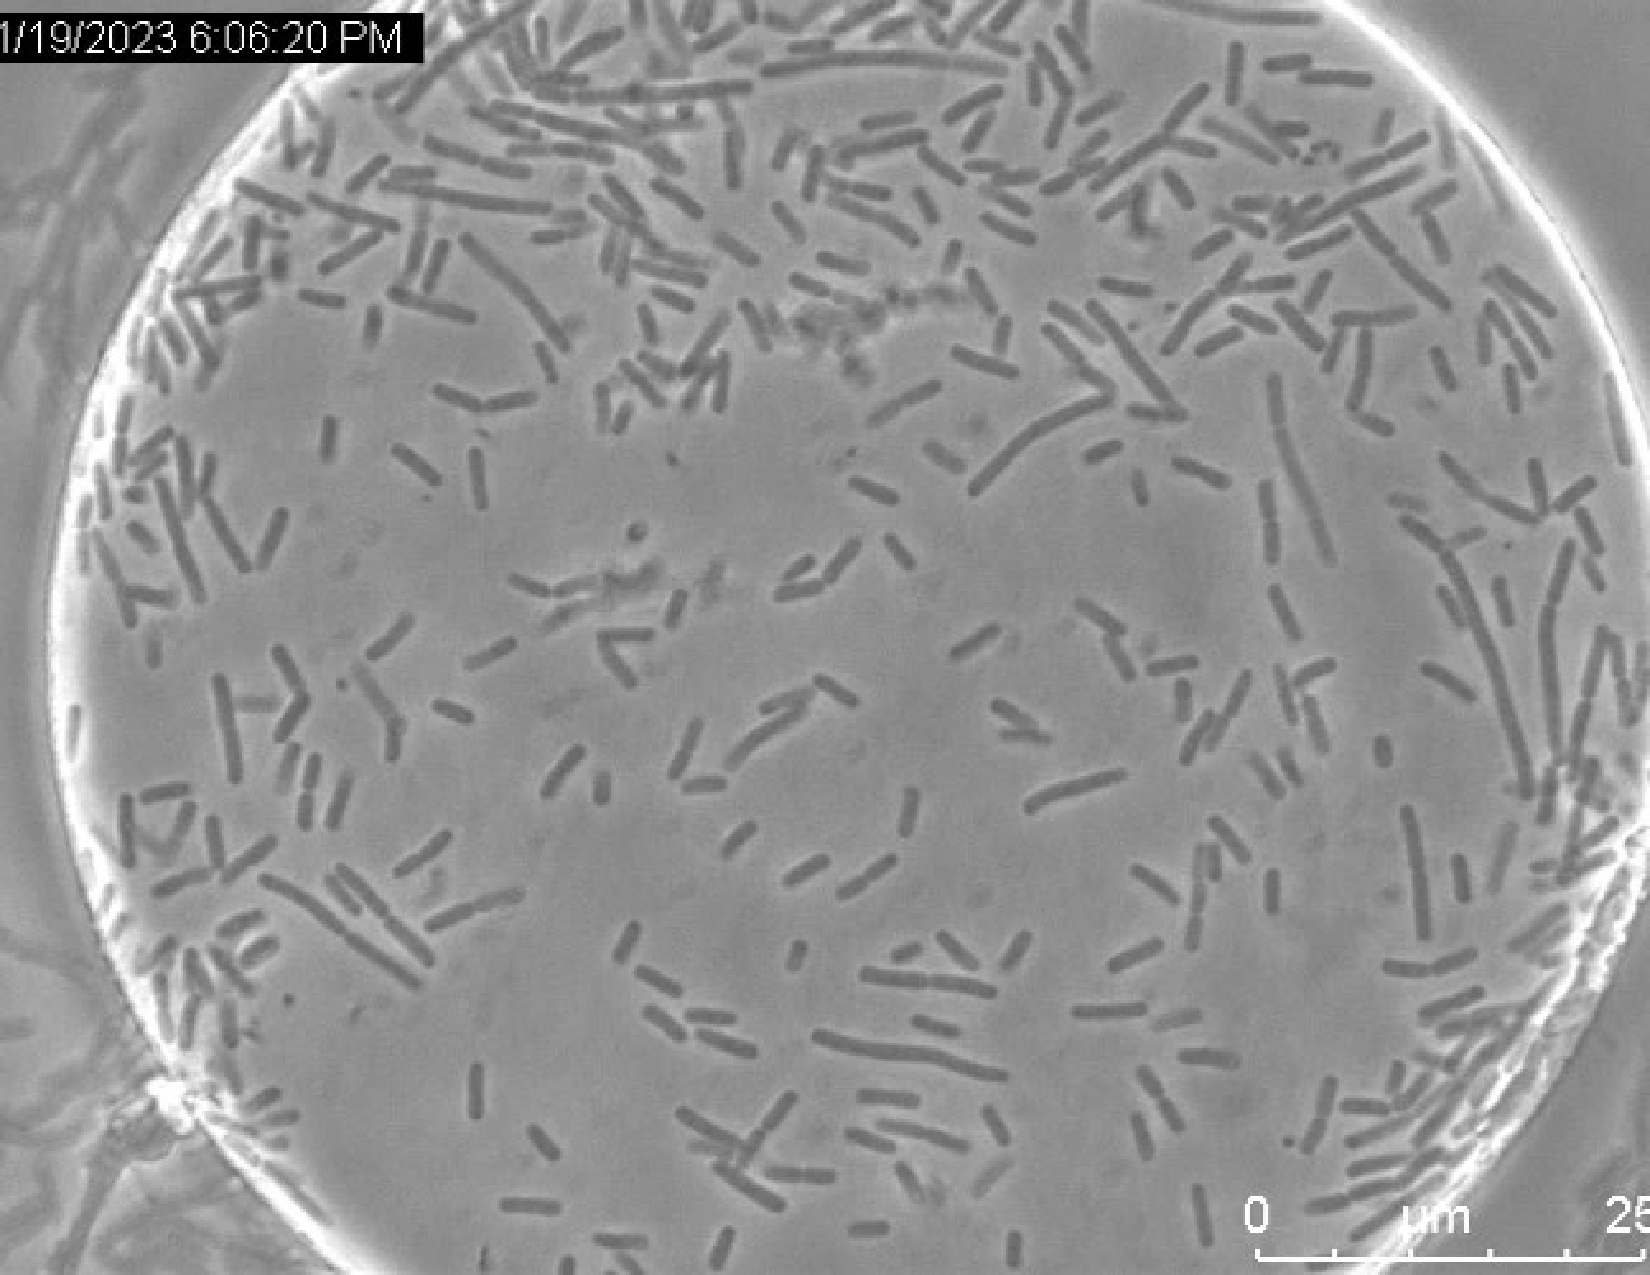
\includegraphics[width=\columnwidth]{Series006_t00000.pdf}
    \subcaption{菌液注入から約4時間20分後.}
    \label{fig:64_1_m9}
  \end{minipage}
  \begin{minipage}{0.45\linewidth}
    \centering
    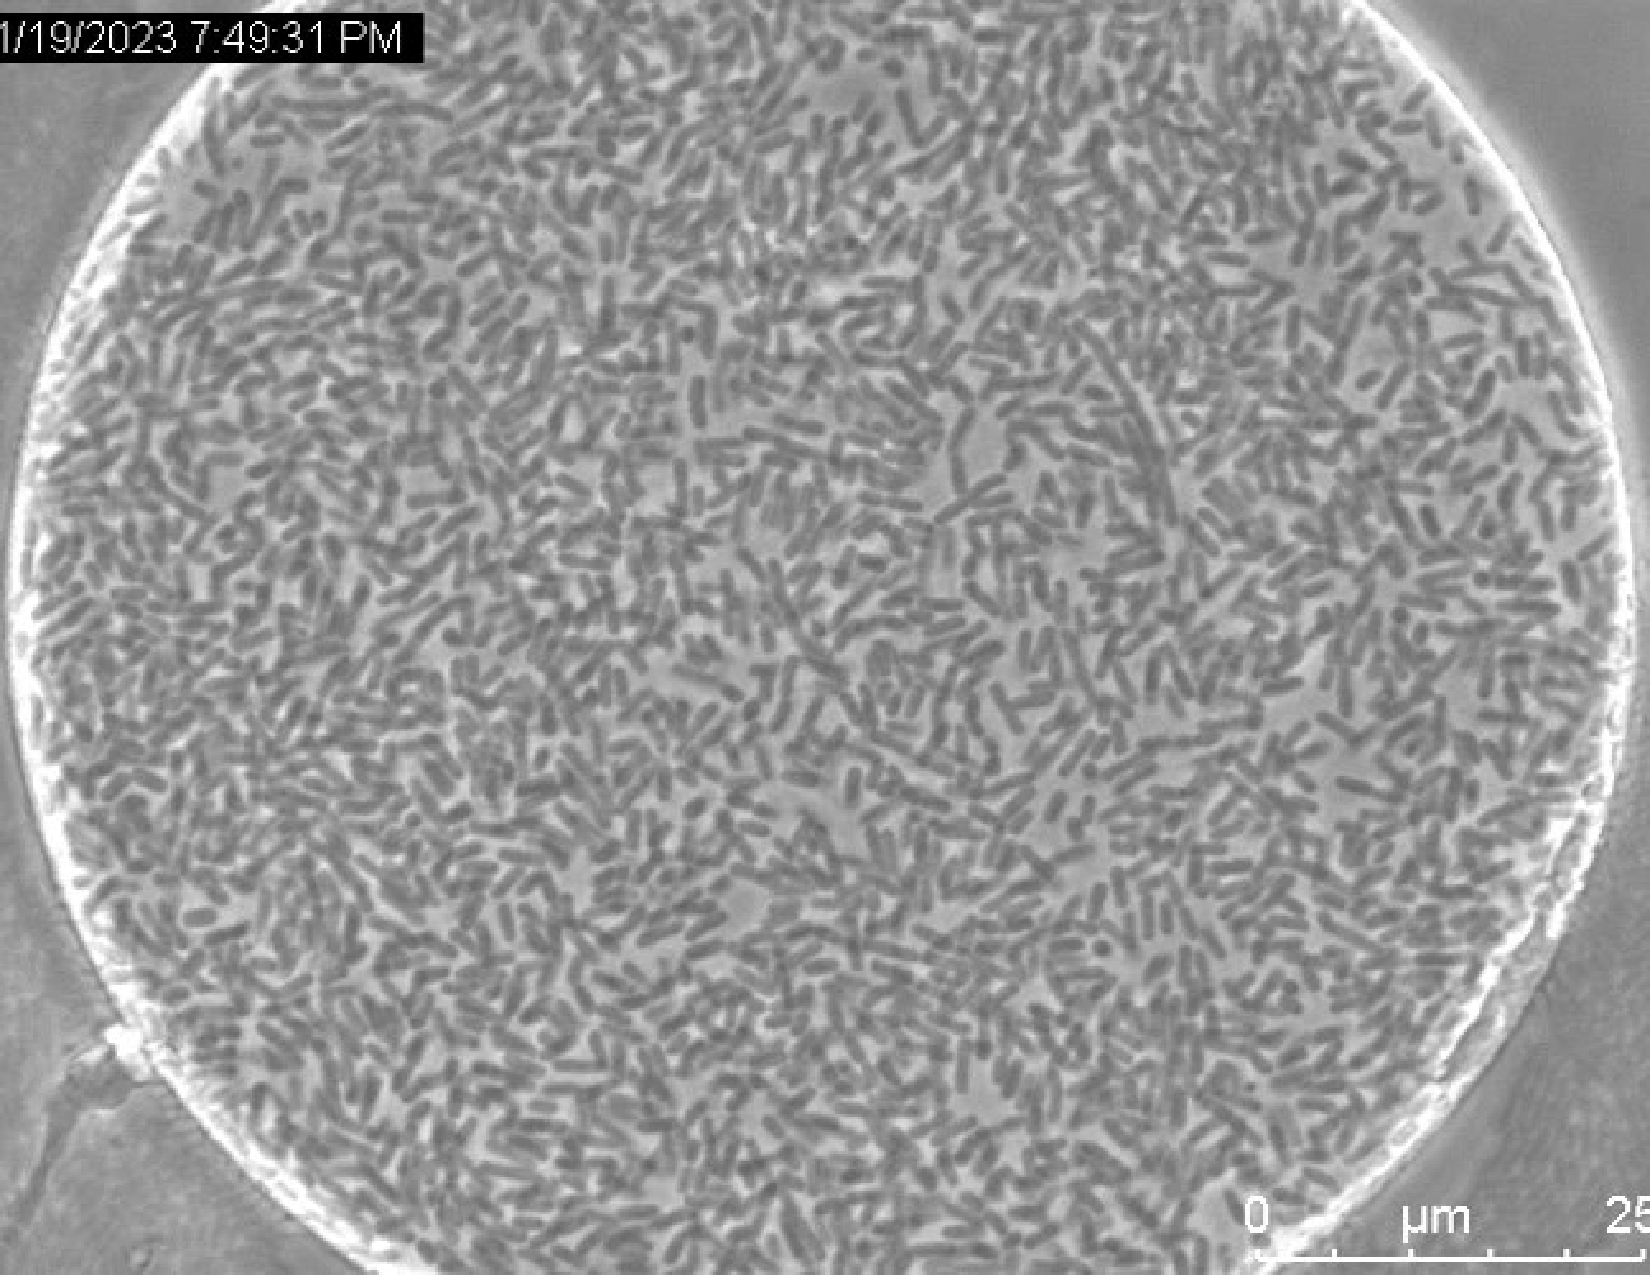
\includegraphics[width=\columnwidth]{Series010_t000000.pdf}
    \subcaption{菌液注入から約6時間10分後.}
    \label{fig:64_2_m9}
  \end{minipage}
  \begin{minipage}{0.45\linewidth}
    \centering
    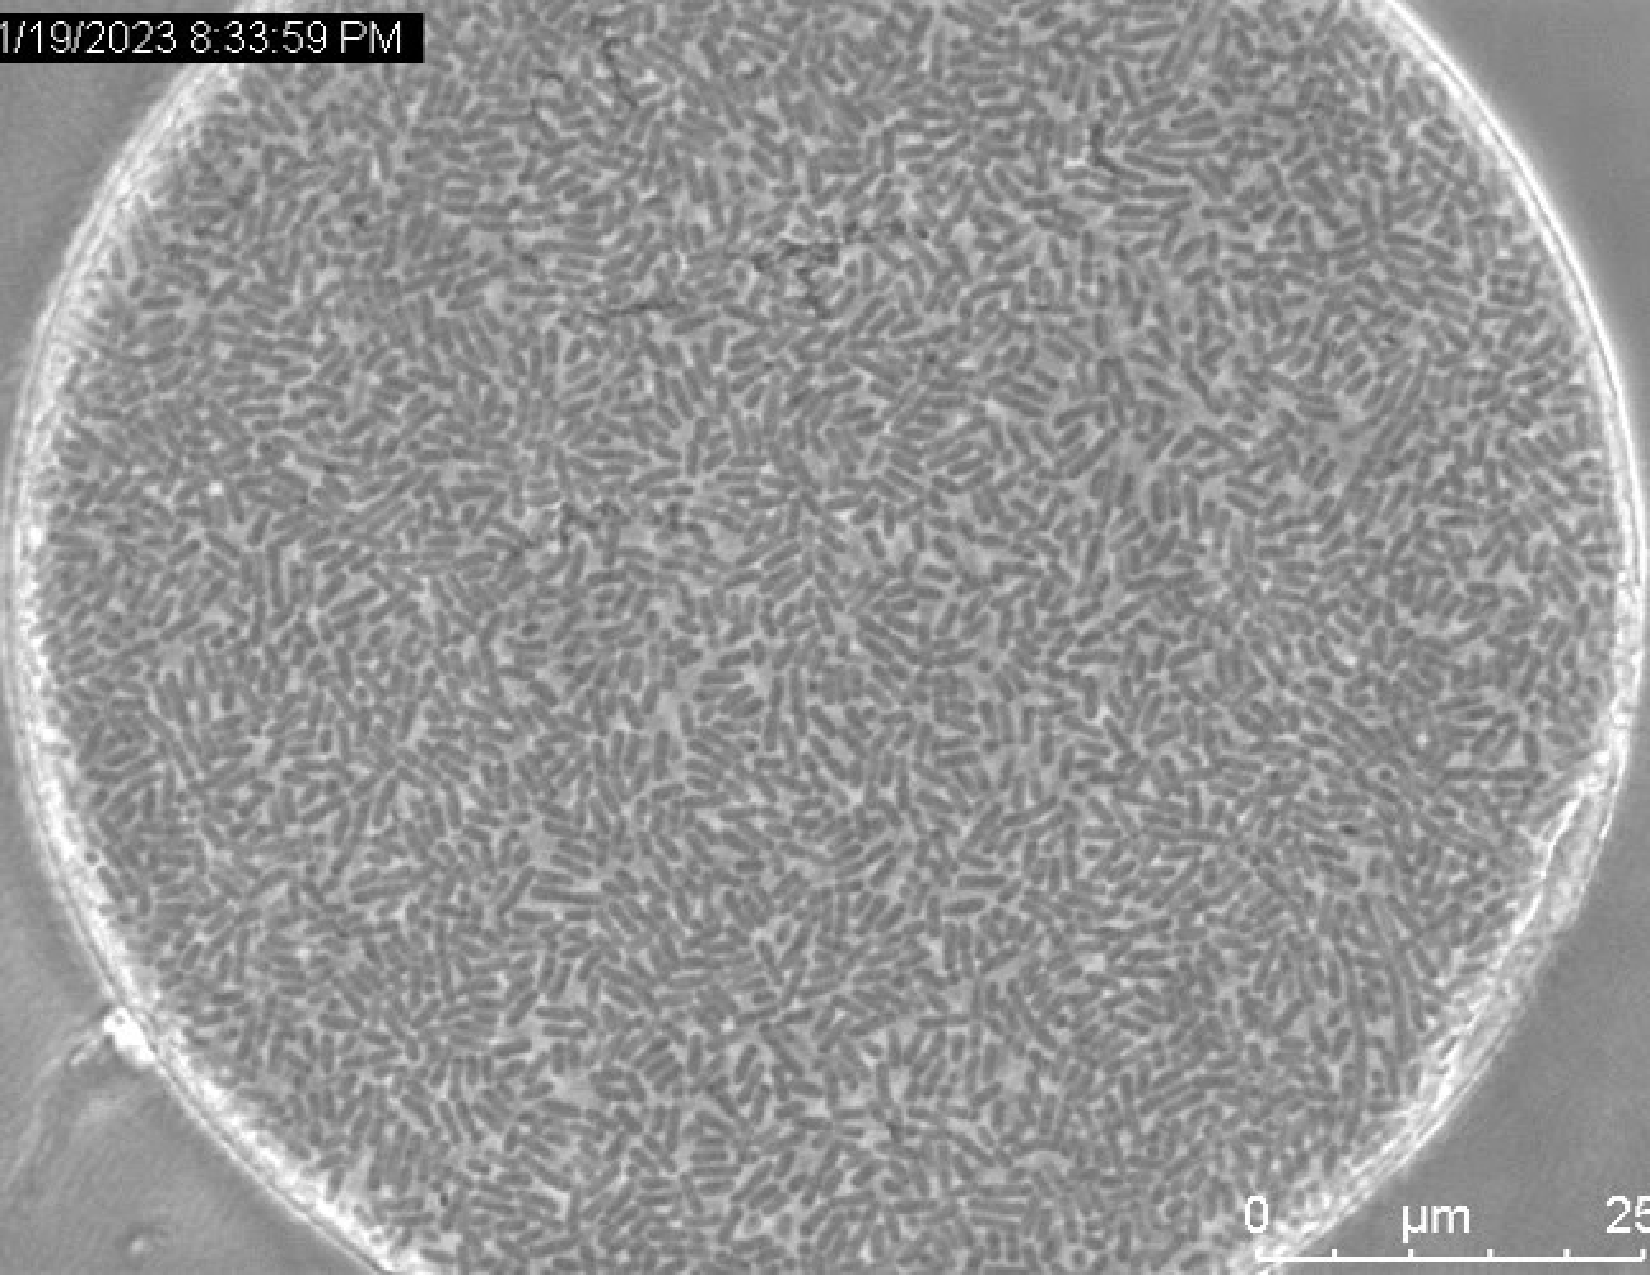
\includegraphics[width=\columnwidth]{Series011_t000000.pdf}
    \subcaption{菌液注入から約6時間50分後.}
    \label{fig:64_3_m9}
  \end{minipage}
  \begin{minipage}{0.45\linewidth}
    \centering
    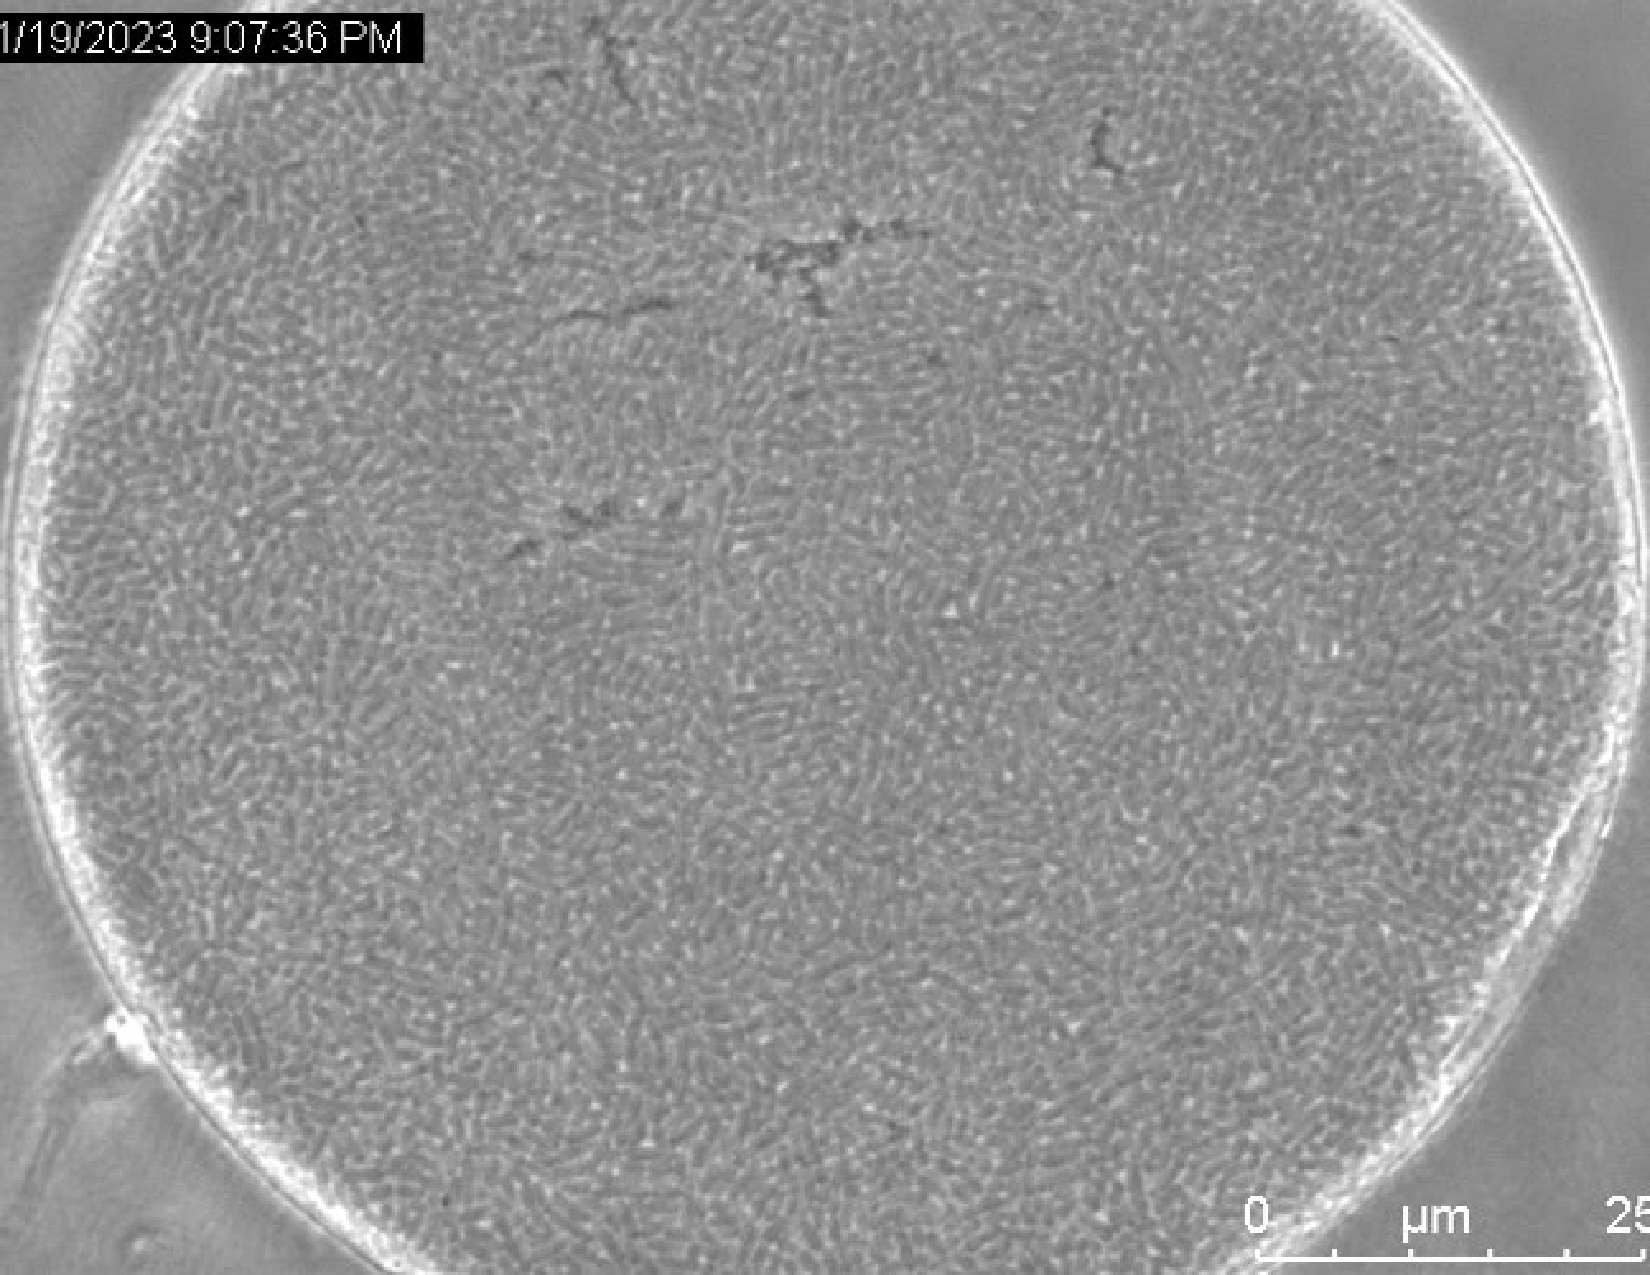
\includegraphics[width=\columnwidth]{Series011_t020000.pdf}
    \subcaption{菌液注入から約7時間30分後.}
    \label{fig:64_4_m9}
  \end{minipage}
  \caption{UU2864を用いた追加実験の結果.左上の時刻表示に合わせると,菌液注入の時刻は13時43分頃である.}
\end{figure}

この実験では,2時間培養後に$\mathrm{OD}_{\SI{600}{nm}}=0.139$となっていた菌液を希釈せず用いた.
観察の結果,まず菌液の注入から約4時間後には菌の大きさはばらついていた(図\ref{fig:64_1_m9}).
しかし,その1,2時間後から長く伸びた個体の減数分裂が進み(図\ref{fig:64_2_m9}),最終的には菌の大きさがほぼ揃った状態でガラス転移が実現した(図\ref{fig:64_3_m9},図\ref{fig:64_4_m9}).
ただし,この実験で観察したウェルの境界のすぐ外側で菌が成長しており,菌の漏れが起こってしまっていた.
この漏れを解消できれば,ウェルの内側に閉じ込められた大腸菌集団のガラス転移をより適切に議論できると考える.

\section{まとめ}
本研究では,タンブリングしない大腸菌の変異株UU2806とUU2864の集団を円形のウェルに閉じ込め,大腸菌の密度の増加によってウェル内をガラス転移させることを試みた.
当初は培地としてTB培地を用い,観察温度を\SI{30}{\degreeCelsius}に保ち,ウェルの直径を\SI{120}{\um}とした実験を行った.
まず,UU2806を用いた実験では,いくつかの個体が繊維状に成長し,ガラス状態の配向場に大きな影響を与えていた.
一方で,UU2864を用いた実験では,繊維状に成長した個体が減数分裂を繰り返したため,ガラス転移を観察できなかった.
この減数分裂を解消するため,培地をM9培地に,観察温度を\SI{37}{\degreeCelsius}に,ウェルの直径を\SI{100}{\um}に変更して追加実験を行った.
その結果,菌のサイズがほぼ均等な状態でのガラス転移が確認できた.
この条件での実験を行うことで,これまで成長に問題があり議論が難しかったタンブリングしない大腸菌のガラス転移を,通常の大腸菌と比較しながら議論できると考える.

\section{謝辞}
本実験を提案してくださり,定期的に研究の方針について議論をしてくださった竹内一将准教授に深く感謝申し上げます.
また,装置の使い方や実験の手順などを丁寧に指導していただき,実験の成功に向けて温かく勇気づけてくださった研究員Hisay Lama博士に心からお礼申し上げます.

\begin{thebibliography}{99}
  \bibitem{glass} 宮崎州正.ガラス転移の統計物理学.(2015).物性研究・電子版,4(4),044206.
  \bibitem{cyto1} Parry, B. R., Surovtsev, I. V., Cabeen, M. T., O’hern, C. S., Dufresne, E. R. and Jacobs-Wagner, C. (2014). The Bacterial Cytoplasm Has Glass-like Properties and Is Fluidized by Metabolic Activity. \textit{Cell}, 156(1-2), 183-194.
  \bibitem{cyto2} Nishizawa, K., Fujiwara, K., Ikenaga, M., Nakajo, N., Yanagisawa, M. and Mizuno, D. (2017). Universal glass-forming behavior of in vitro and living cytoplasm. \textit{Scientific Reports}, 7(1).
  \bibitem{lama} Lama, H., Yamamoto, M. J., Furuta, Y., Shimaya, T. and Takeuchi, K. A. (2022). Emergence of bacterial glass: two-step glass transition in 2D bacterial suspension. \\
  \url{https://doi.org/10.48550/arXiv.2205.10436}
  \bibitem{emps} Shimaya, T., Okura, R.,  Wakamoto Y. and Takeuchi, K. A. (2021). Scale invariance of cell size fluctuations in starving bacteria. \textit{Communications Physics}, 4(238).  
\end{thebibliography}

\end{document}